% -*- coding: utf-8 -*-
%%%%%%%%%%%%%%%%%%%%%%%%%%%%%%%%%%%%%%%%%%%%%%%%%%%%%%%%%%%%%%%%%%%%%%%%%%%%%%%%
%2345678901234567890123456789012345678901234567890123456789012345678901234567890
%        1         2         3         4         5         6         7         8

%\UseRawInputEncoding


\documentclass[letterpaper, 10 pt, conference]{ieeeconf}  % Comment this line out if you need a4paper

%\pdfminorversion=4              % tell pdflatex to generate PDF in version 1.4
\usepackage[T1]{fontenc}
\usepackage{amssymb}
\usepackage{graphicx}
\usepackage{subfigure}
\usepackage{mathtools}
\usepackage{multirow,makecell}
\usepackage{caption}
%\documentclass[a4paper, 10pt, conference]{ieeeconf}      % Use this line for a4 paper

\IEEEoverridecommandlockouts                              % This command is only needed if 
                                                          % you want to use the \thanks command

\overrideIEEEmargins                                      % Needed to meet printer requirements.

%In case you encounter the following error:
%Error 1010 The PDF file may be corrupt (unable to open PDF file) OR
%Error 1000 An error occurred while parsing a contents stream. Unable to analyze the PDF file.
%This is a known problem with pdfLaTeX conversion filter. The file cannot be opened with acrobat reader
%Please use one of the alternatives below to circumvent this error by uncommenting one or the other
%\pdfobjcompresslevel=0
%\pdfminorversion=4

% See the \addtolength command later in the file to balance the column lengths
% on the last page of the document

% The following packages can be found on http:\\www.ctan.org
%\usepackage{graphics} % for pdf, bitmapped graphics files
%\usepackage{epsfig} % for postscript graphics files
%\usepackage{mathptmx} % assumes new font selection scheme installed
%\usepackage{times} % assumes new font selection scheme installed
%\usepackage{amsmath} % assumes amsmath package installed
%\usepackage{amssymb}  % assumes amsmath package installed
\usepackage{cite}

\title{\LARGE \bf
Recurrent Neural Networks for Range-based Indoor Robot Localization}


\author{Hyungtae Lim$^{1}$ , Jungmo Koo$^{2}$, Jieum Hyun$^{3}$, Hyun Myung$^{4}$, \textit{Senior Member, IEEE}% <-this % stops a space
\thanks{
	*This material is based upon work supported by the Ministry of Trade, Industry \& Energy(MOTIE, Korea) under Industrial Technology Innovation Program. No.10067202, 'Development of Disaster Response Robot System for Lifesaving and Supporting Fire Fighters at Complex Disaster Environment'.}% <-this % stops a space
\thanks{$^{1}$Hyungtae Lim, $^{2}$Jungmo Koo, $^{3}$Jieum Hyun, and $^{4}$Hyun Myung are with
	the Urban Robotics Laboratory, Korea Advanced Institute of Science
	and Technology (KAIST) Daejeon, 34141, South Korea. {\tt\small \{shapelim, jungmokoo, jimi, hmyung\}@kaist.ac.kr}}%
%
}


\begin{document}

\captionsetup[figure]{labelformat={default},labelsep=period,name={Fig.}}


\maketitle
\thispagestyle{empty}
\pagestyle{empty}


%%%%%%%%%%%%%%%%%%%%%%%%%%%%%%%%%%%%%%%%%%%%%%%%%%%%%%%%%%%%%%%%%%%%%%%%%%%%%%%%
\begin{abstract}

Range-only SLAM is a method for localizing a mobile robot and beacons by mainly utilizing distance measurements. Unlike the traditional probability-based range-only SLAM method, we present a novel approach using a recurrent neural network architecture that directly learns the end-to-end mapping between distance data and robot position.

\end{abstract}


%%%%%%%%%%%%%%%%%%%%%%%%%%%%%%%%%%%%%%%%%%%%%%%%%%%%%%%%%%%%%%%%%%%%%%%%%%%%%%%%
\section{INTRODUCTION}

 As deep learning age has come, various kinds of deep neural architectures have been proposed for many tasks. Especially, recurrent neural networks (RNNs) have been shown to achieve better performance in case of dealing with time variant information, such as not only speech recognition, but also pose estimation and robot localization, than traditional methods. 
 
In this poster, we tested various kinds of RNN models for robot localization using range data. We trained 4 kinds of RNNs; LSTM\cite{hochreiter1997long}, GRU\cite{cho2014learning}, Bi-LSTM\cite{schuster1997bidirectional}, stacked Bi-LSTM, which are basic architecture units of many RNNs. Using deep learning, these structures directly learn the end-to-end mapping between distance data and robot position. 

\begin{figure}[h]
	
	\centering
	%\subfigure[]{
		%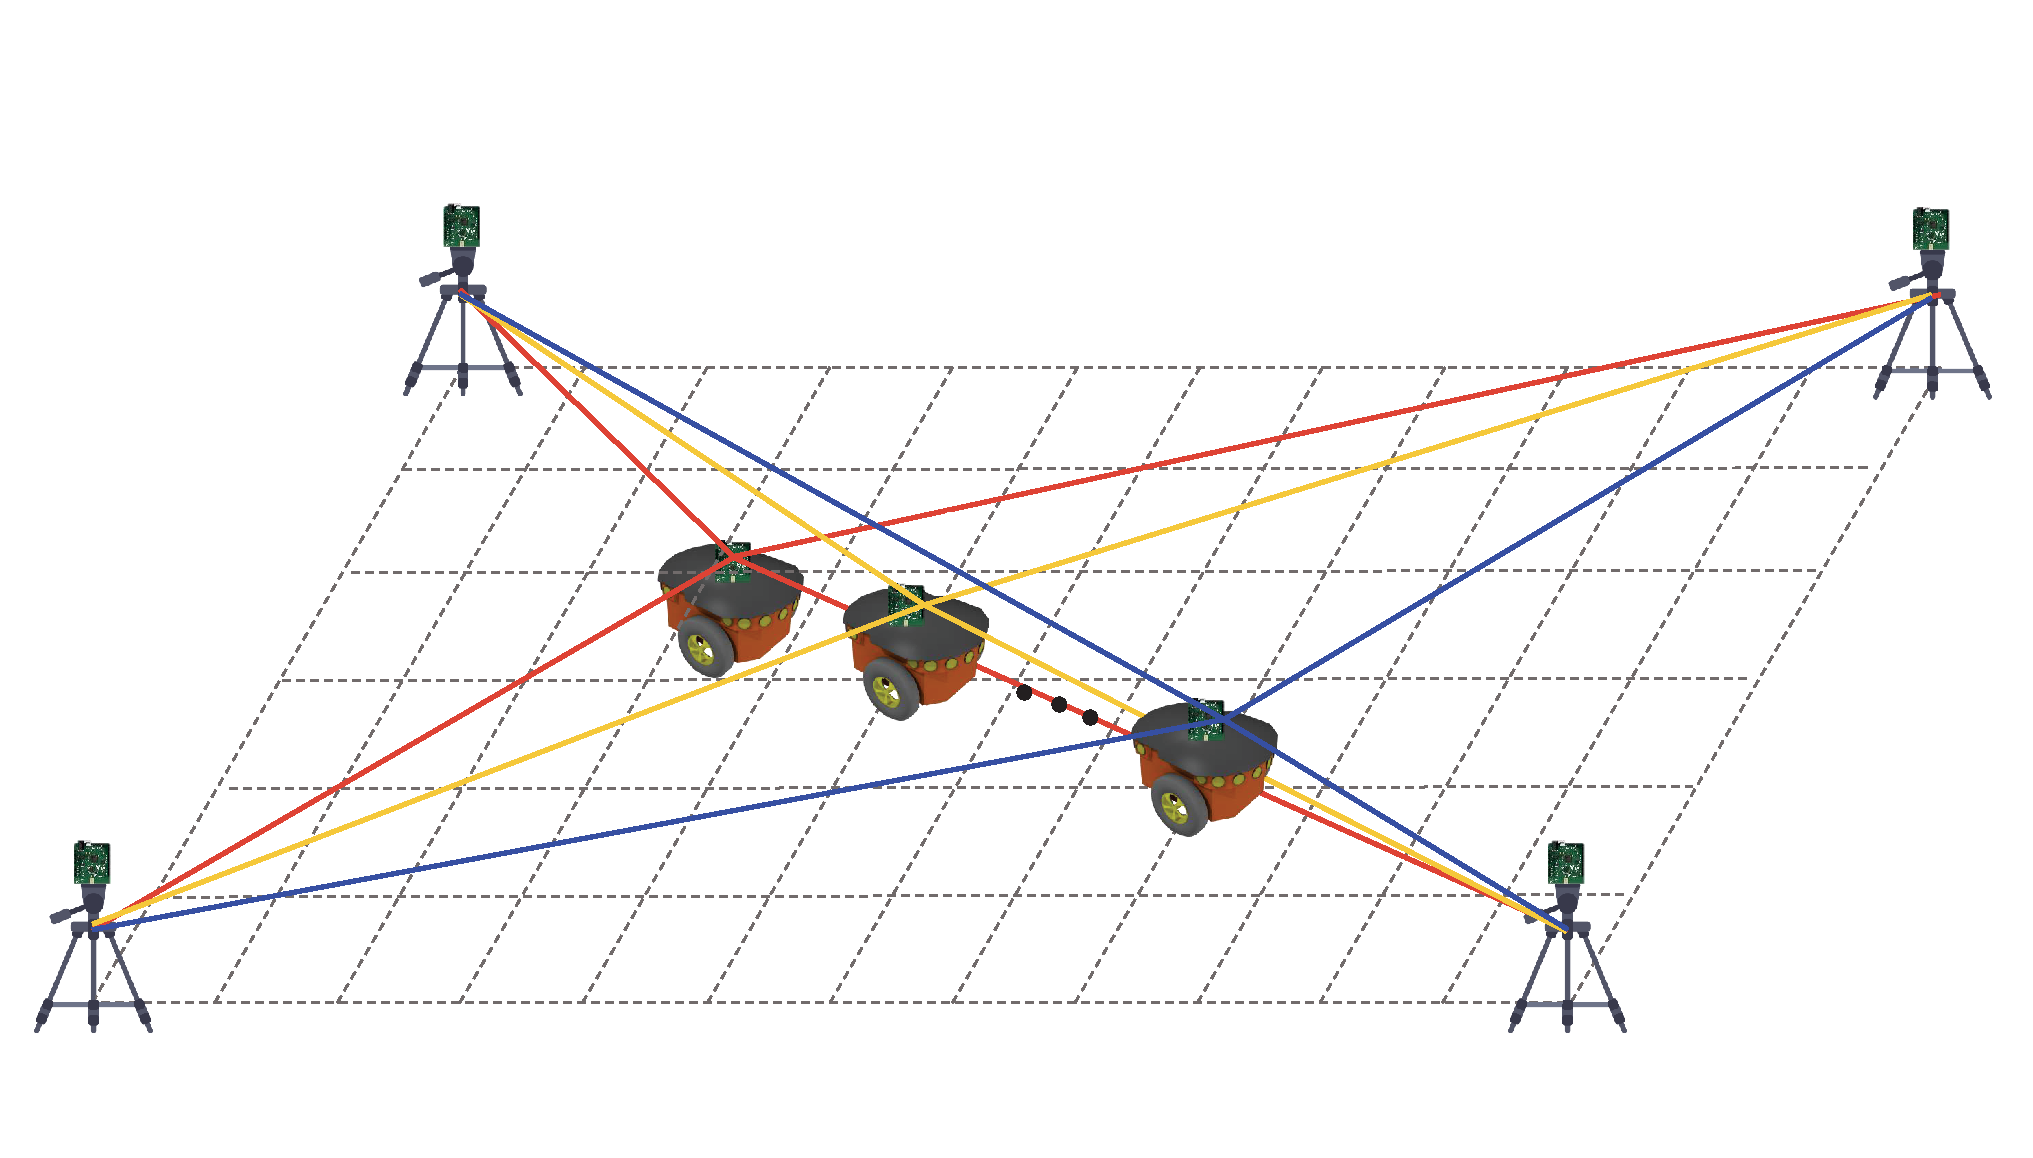
\includegraphics[height=4.5cm]{IROS2018_image_1}
	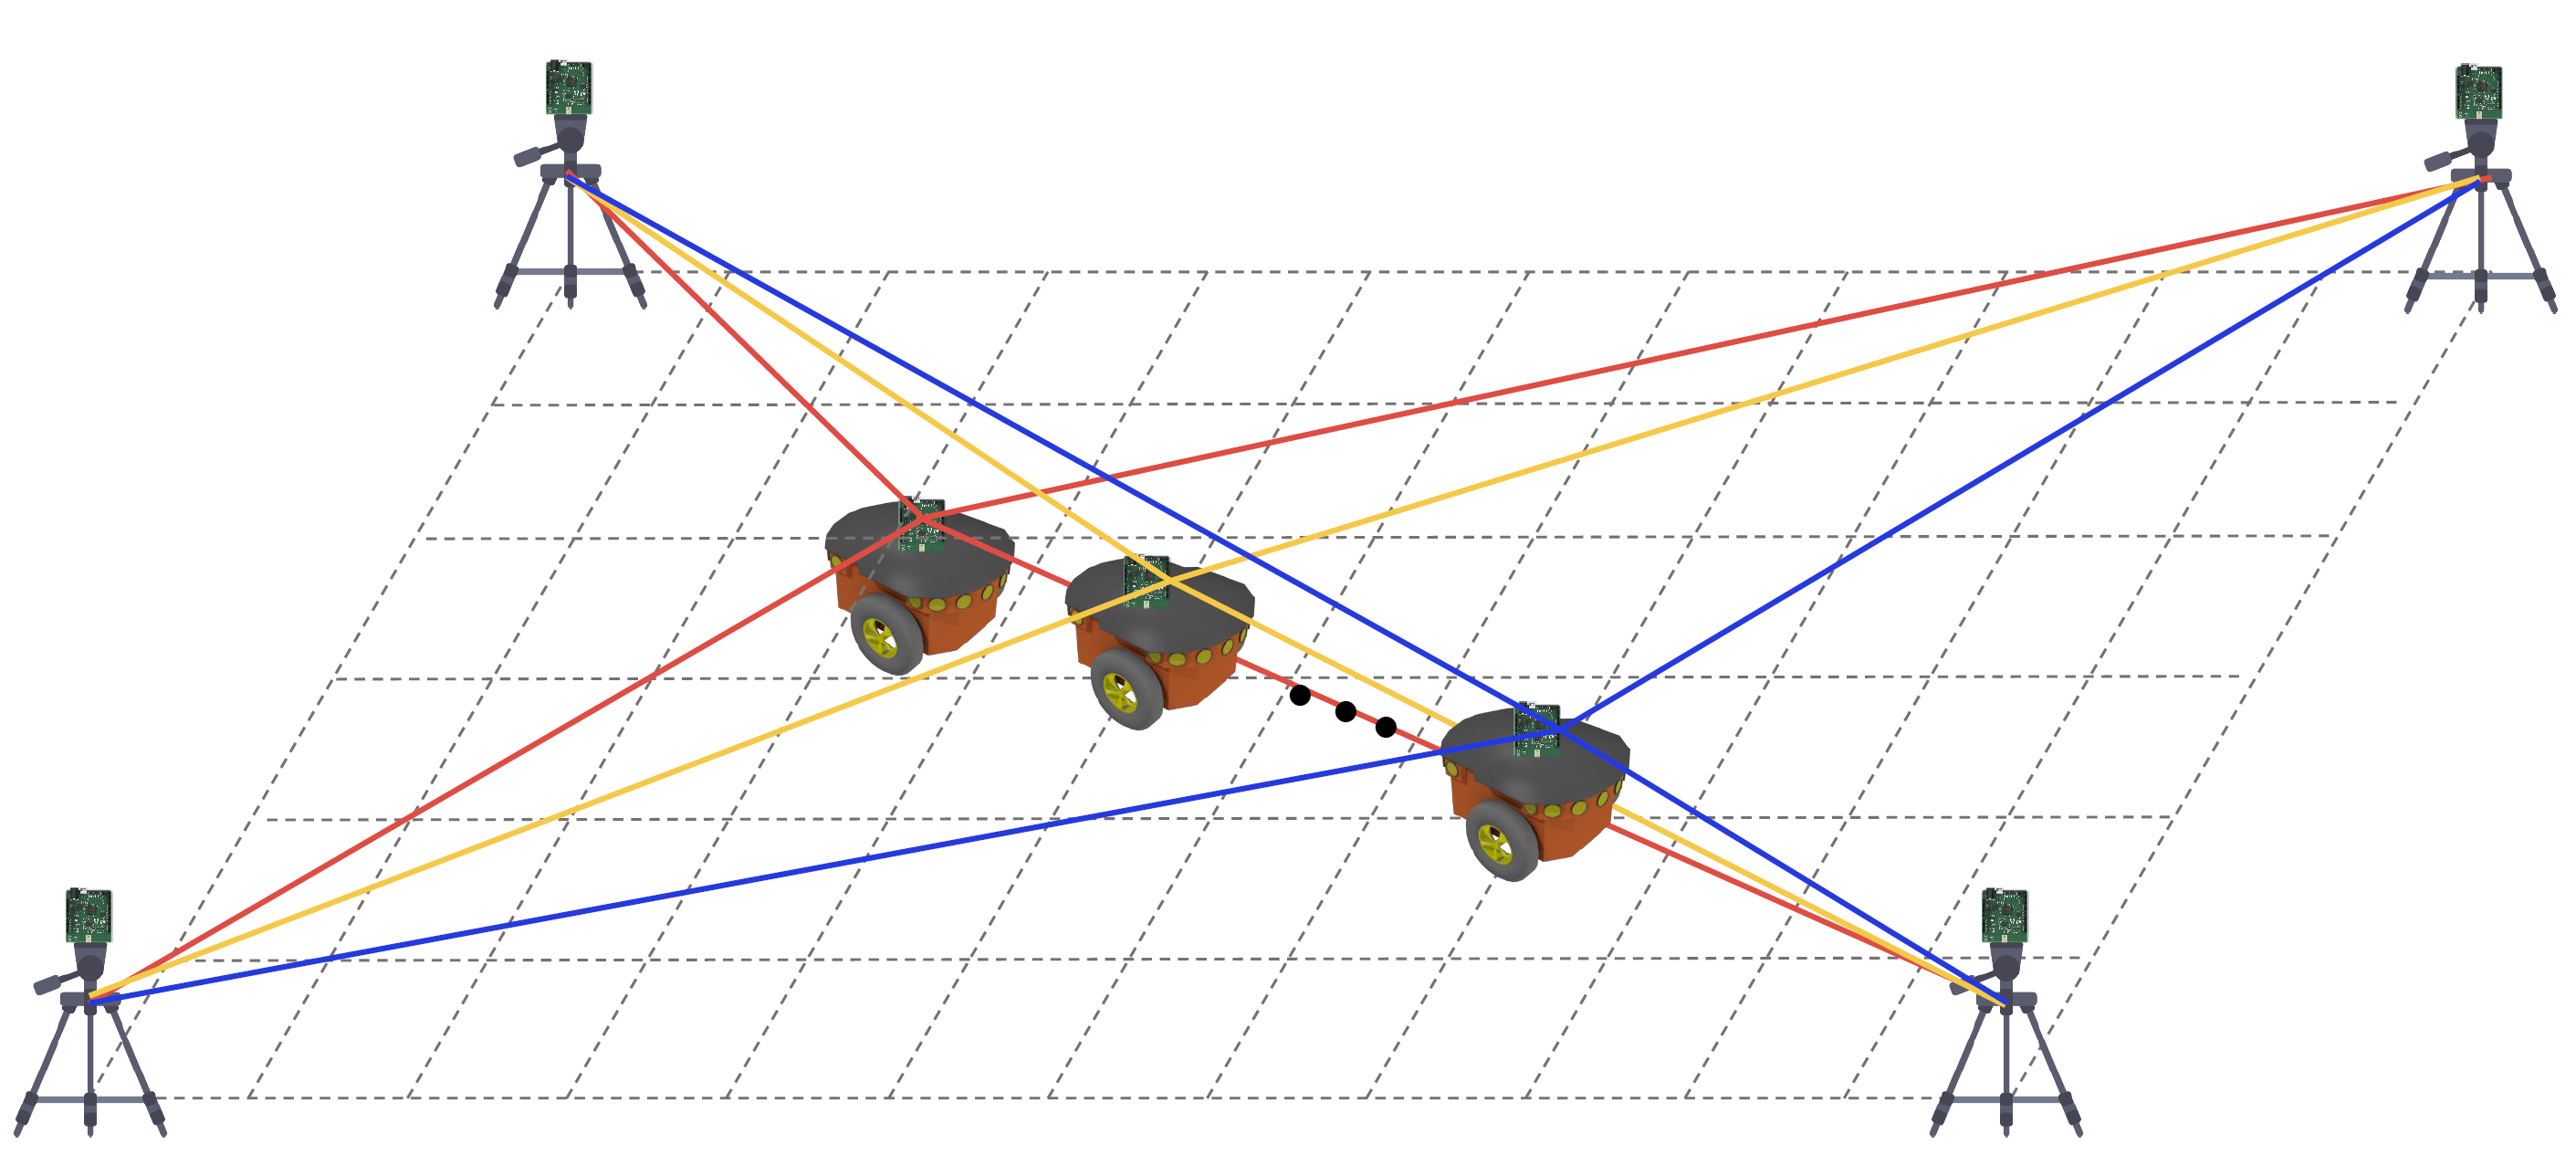
\includegraphics[height=3.0cm]{overview}
		
		%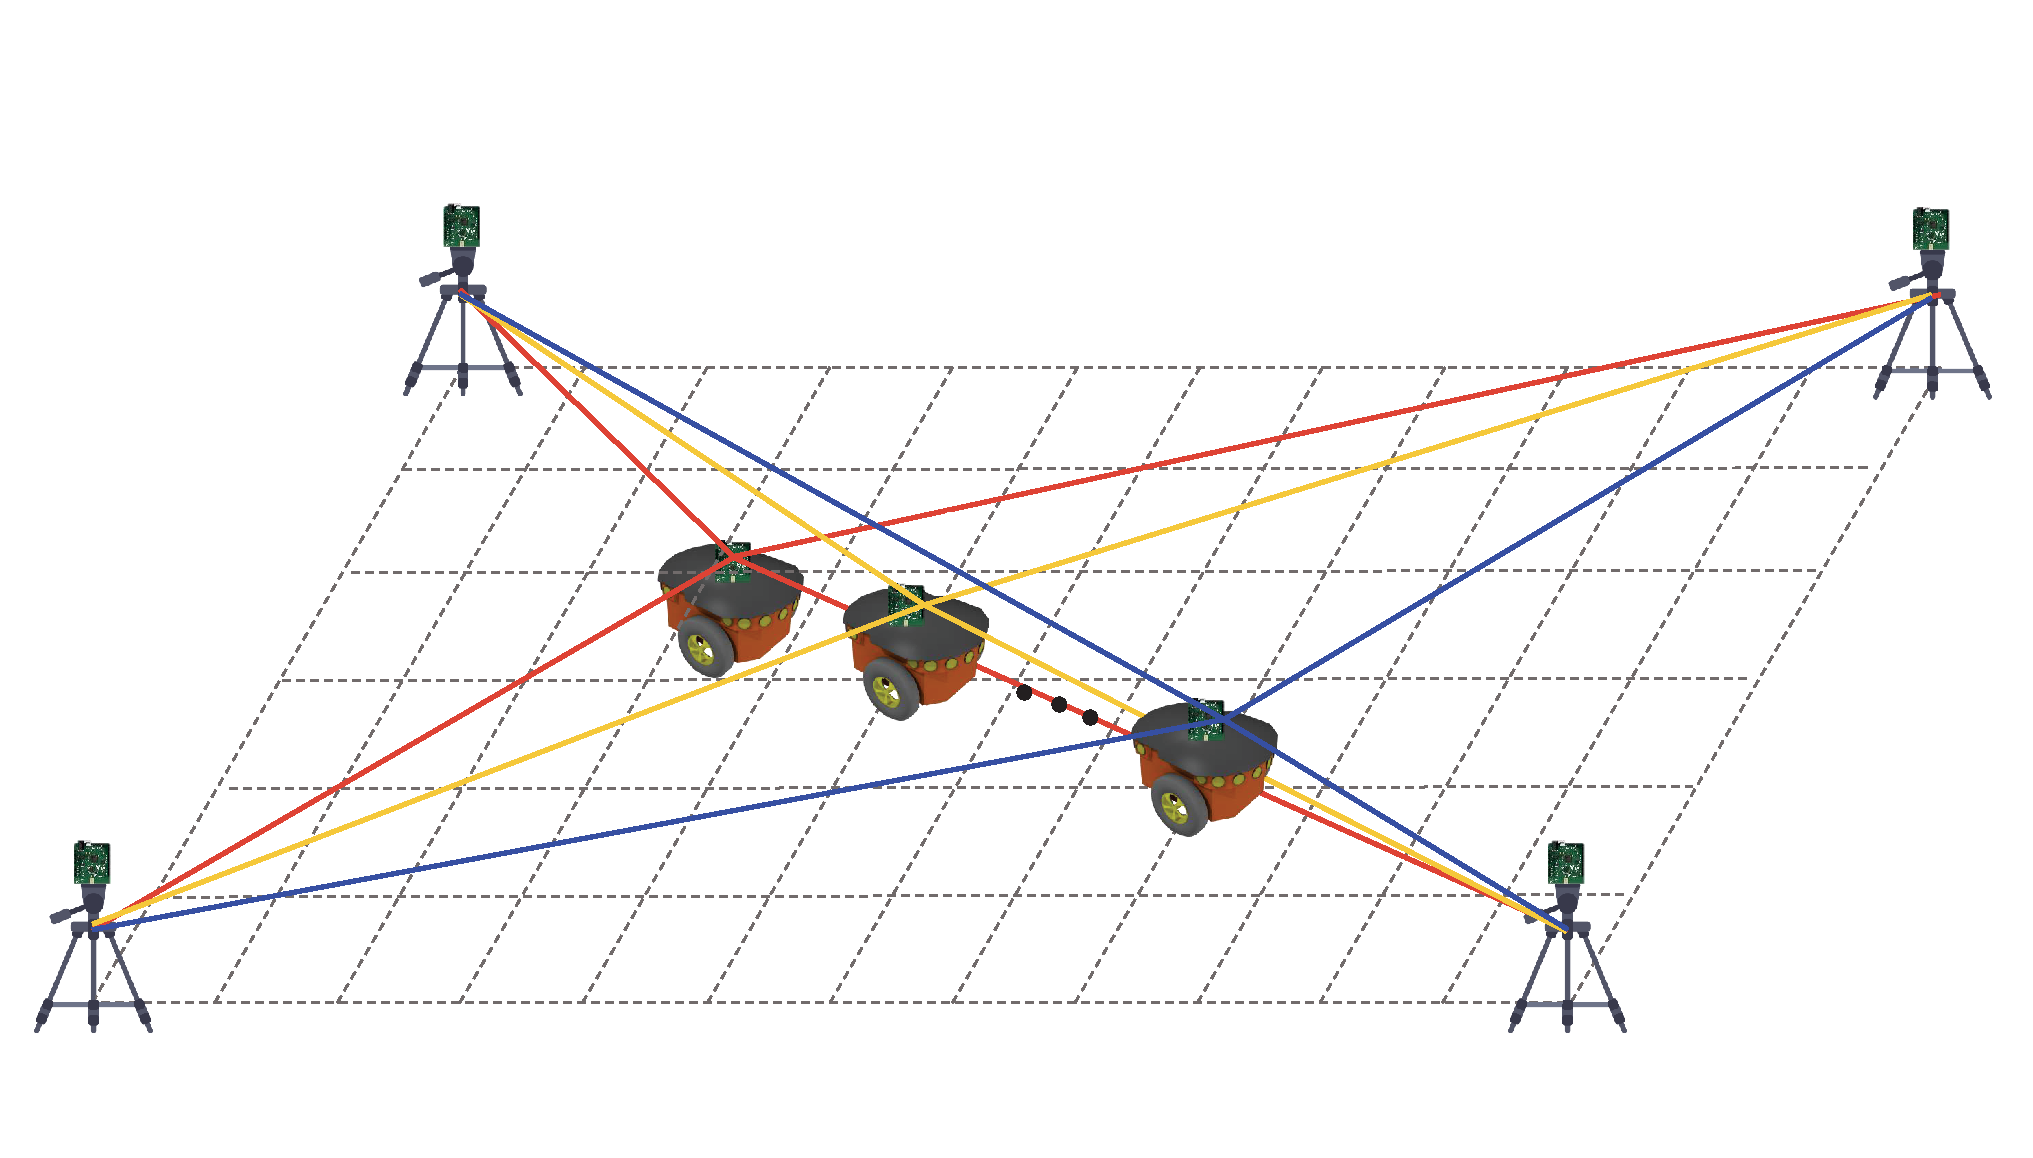
\includegraphics[trim={0 0 0 1cm}height=4.5cm]{IROS2018_image_1}
	\label{fig:example}
%	}

	\caption{System overview. A robot localizes its own pose through distance data and the derivative of distance data. }
	
\end{figure}
\section{Experiment}

 We set the experiment on the virtual situation and generate distance data set which corresponds to the position with 10\% noise error and let RNN be trained using these distance data. Train data are just zigzag paths and test data is an arbitrary path, so we also check if RNN can estimate the position despite the variation of distance data as input.
   
 Let $\Theta$ be the parameters of our RNN model, then our final goal is to find optimal parameters $\Theta^{*}$ for localization by minimizing Mean Square Error (MSE) of Euclidean distance between ground truth position $Y_k$ and estimated position $\hat{Y_k}$.
\begin{equation}
\Theta^{*} = \underset{\Theta}{\mathrm{argmin}} \sum_{k=1}^N \parallel Y_k - \hat{Y_k} \parallel^{2}
\end{equation}  

\section{Results}
 
 The prediction of trajectory results are shown in Fig. \ref{fig:example2} and Root-Mean-Squared Error (RMSE) are shown in Table \ref{table:rmse}. As a result, the stacked Bi-LSTM showed better performance than the other RNNs. Therefore, we can conclude that the performance improves as the nonlinearity of the architecture increases.
 
\begin{figure}[h]
	
	\centering
	\subfigure[]{
		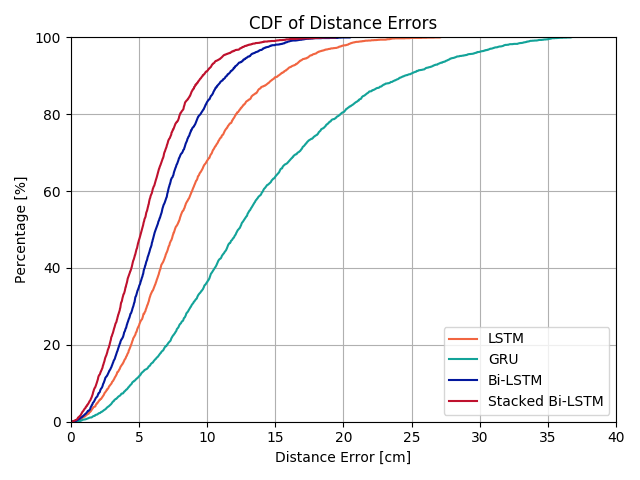
\includegraphics[height=3cm]{cdf_distance_error_graph}
		\label{fig:example}
	}
	\subfigure[]{
		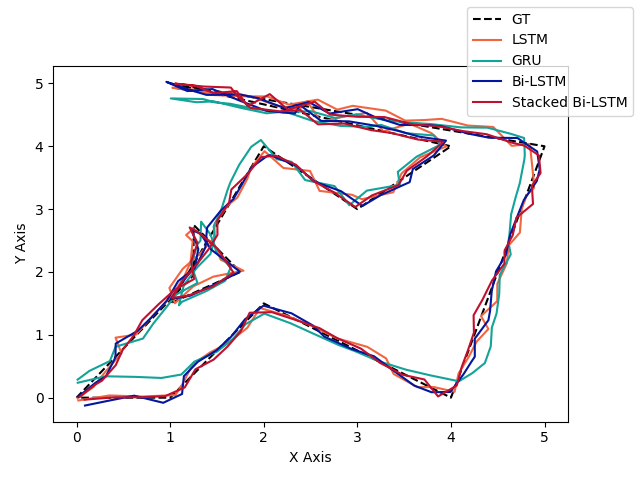
\includegraphics[height=3cm]{2d_trajectory}
		\label{fig:example2}	
	}	
	\caption{ (a) CDF of distance errors gragh (\textit{The trial that reaches 100\% faster is better}) (b) trajectory results of RNNs. .}
	
\end{figure}

\begin{table}[h]
	\centering
	\caption{RMSE of each RNN model from the test data.}
	\begin{tabular}{cccc}
		\hline
		\multicolumn{4}{c}{RMSE of Localization {[}cm{]}}                                          \\ \hline
		LSTM                 & GRU              & Bi-LSTM                  & Stacked Bi-LSTM        \\
		9.6839               & 15.5183              & 7.5110                    & \textbf{6.3788}                    \\ \hline
		\multicolumn{1}{l}{} & \multicolumn{1}{l}{} & \multicolumn{1}{l}{} & \multicolumn{1}{l}{}
		
	\end{tabular}
	
	\label{table:rmse}
	
\end{table}

\section{Conclusions}

We suggested a novel approach to range-based localization using recurrent neural network models. Results show that the RNN-based localization can reduce position error. As a future work, RNNs need to be tested in the real-world

\bibliographystyle{IEEEtran}
% argument is your BibTeX string definitions and bibliography database(s)
\bibliography{./IEEEabrv,./MyBib}


\end{document}
